\documentclass[12pt,article]{article}
\usepackage{fullpage}
\usepackage[top=2cm, bottom=4.5cm, left=2cm, right=2cm]{geometry}
\usepackage{amsmath,amsthm,amsfonts,amssymb,amscd}
\usepackage{lastpage}
\usepackage{enumerate}
\usepackage{fancyhdr}
\usepackage{mathrsfs}
\usepackage{xcolor}
\usepackage{graphicx}
\usepackage{listings}
\usepackage{hyperref}
\usepackage{mdframed}
\usepackage{changepage}   % for the adjustwidth environment
\usepackage{forest} 
\usepackage{tikz}   % For graph

\usepackage{float}  % To inforce inserting images at the right place


\newcommand{\Tau}{\mathrm{T}}

\DeclareMathOperator*{\argmax}{arg\,max}
\DeclareMathOperator*{\argmin}{arg\,min}

% For matrix
\def\horzbar{\text{magic}}

\hypersetup{%
  colorlinks=true,
  linkcolor=blue,
  linkbordercolor={0 0 1}
}

\setlength{\parindent}{0.0in}
\setlength{\parskip}{0.05in}

\newcommand\projnumber{1}
\newcommand\course{CS534}
\newcommand\OSUID{934370552}
\newcommand\Email{buivy@oregonstate.edu}
\newcommand\Name{Vy Bui}
\newcommand\tab[1][1cm]{\hspace*{#1}}

\pagestyle{fancyplain}
\headheight 35pt
\lhead{Homework Assignment \projnumber}
\rhead{Oct. 14, 2022}
\lfoot{}
\cfoot{}
\rfoot{\small\thepage}
\headsep 1.5em

\newenvironment{problem}[2][Problem]
    { \begin{mdframed}[backgroundcolor=gray!20] \textbf{#1 #2} \\}
    {  \end{mdframed}}
   

% Make Rightarrow with superscript
\makeatletter
\newcommand{\xRightarrow}[2][]{\ext@arrow 0359\Rightarrowfill@{#1}{#2}}
\makeatother

\begin{document}

\begin{titlepage}
    \begin{center}
        \vspace*{4cm}

        \textbf{\Large CS534 - Machine Learning}

        \vspace{0.5cm}
 
        \textbf{\Large Written Homework Assignment \projnumber{}}
 
        \vspace{1cm}

        Author: Vy Bui

        OSUID: 934370552 \\ 
        
        Email: buivy@oregonstate.edu

        \vfill
             
        \vspace{0.8cm}
      
             
        The School of Electrical Engineering and Computer Science\\
        Oregon State University\\
             
    \end{center}
\end{titlepage}

%==============================================================================%
\begin{problem}{1}
\textbf{[10pts]}
\end{problem}

\textbf{(a)} The log likelihood function of \textbf{w} is 

$$l(w) = log\prod_{i=1}^{N} P(y_i | \mathbf{x_i; w})$$

\textbf{(b)} \newline
First, maximizing the log likelihood function is equivalent to minimizing the 
negative log likelihood function.

$$\argmax_{w} log(w) = \argmin_{w} -log(w) 
= \argmin_{w} -log\prod_{i=1}^{N} P(y_i | \mathbf{x_i; w})
= \argmin_{w} -\sum_{i=1}^{N} log p(y_i | \mathbf{x_i; w}) \tab[0.5cm] (1)$$

Because the likelyhood is Gaussian,
$$log p(y_i | \mathbf{x_i; w}) = -\frac{(y_i - \mathbf{x_i^Tw})^2}{2\sigma^2} + const \tab[1cm] (2)$$

where the const consists of all terms independent of $\mathbf{w}$.

Substituting (2) to (1) and droping const results in

$$\argmax_{w} log(w) 
= \argmin_{w} -\sum_{i=1}^{N} log p(y_i | \mathbf{x_i; w})
= \argmin_{w} \sum_{i=1}^{N} \frac{(y_i - \mathbf{x_i^T w})^2}{2\sigma^2}
$$

$$
= \frac{1}{2} \sum_{i=1}^{N} a_i (\mathbf{w^T x_i} - y_i)^2, a_i = \frac{1}{\sigma^2} \tab[1cm] (3)
$$ 

\textbf{(c)}
The gradient of $L(\mathbf{w})$ can be computed as following

$$
\nabla L(w) = \frac{1}{\sigma^2} \sum_{i=1}^{N} (\mathbf{w^T x_i} - y_i) \mathbf{x_i}
$$

Because the gradient points in the direction of steepest ascent, we need to 
go in the opposite direction to reach the minimum, one step at a time. Hence, 
the update rule is 

$$
\mathbf{w \leftarrow w} - \gamma \nabla L(w) = \mathbf{w} - \frac{1}{\sigma^2} \sum_{i=1}^{N} (\mathbf{w^T x_i} - y_i) \mathbf{x_i}
$$

\textbf{(d)}
Because (3) is a quadratic function of \textbf{w}, we can compute the global 
optimum by setting its gradient to 0 and solve for \textbf{w}.

$$
\frac{\ l}{\partial \mathbf{w}} 
= \frac{1}{2\sigma^2} \frac{d}{d\mathbf{w}} (\mathbf{(y - xw)^T (y - xw)})
= \frac{1}{2\sigma^2} \frac{d}{d\mathbf{w}} (\mathbf{(y^Ty -2y^Txw + w^Tx^Txw)})
$$

$$
= \frac{1}{2\sigma^2} \frac{d}{d\mathbf{w}} (\mathbf{(-y^TX + w^Tx^Tx)}) \tab[1cm] (4)
$$

Setting (4) to 0 results in

$$
\mathbf{w_{op}^Tx^Tx = y^TX}
\Leftrightarrow
\mathbf{w_{op}^T = y^Tx(x^Tx)^{-1}}
\Leftrightarrow
\mathbf{w_{op} = (x^Tx)^{-1}x^Ty}
$$

%==============================================================================%
\newpage
\begin{problem}{2}
\textbf{[10pts]}
\end{problem}

\textbf{(a)} Compute the log-likelihood function \newline
$$
l(w) = log L(w) = \sum_{i=1}^{N} \sum_{k=1}^{K} log(p(y = k| x_i)^{y_{ik}})
= \sum_{i=1}^{N} \sum_{k=1}^{K} log(\frac{e^{\mathbf{w_k^T x_i}}}{\sum_{j=1}^{K} e^{\mathbf{w_j^T x_i}}}) ^ {y_{ik}}
$$

\textbf{(b)} Compute the gradient of the log-likelihood function with regard to 
the weight vector $\mathbf{w}_c$ of class c.

First, the function can be simplified as follows

$$
l(w) = \sum_{i=1}^{N} \sum_{k=1}^{K} log(\frac{e^{\mathbf{w_k^T x_i}}}{\sum_{j=1}^{K} e^{\mathbf{w_j^T x_i}}}) ^ {y_{ik}}
= \sum_{i=1}^{N} \sum_{k=1}^{K} y_{ik} log(\frac{e^{\mathbf{w_k^T x_i}}}{\sum_{j=1}^{K} e^{\mathbf{w_j^T x_i}}})
$$

$$
= \sum_{i=1}^{N} \sum_{k=1}^{K} y_{ik} (\mathbf{w_k^T x_i} - log \sum_{j=1}^{K} e^{\mathbf{w_j^T x_i}})
= \sum_{i=1}^{N} (\sum_{k=1}^{K} y_{ik} \mathbf{w_k^T x_i} - \sum_{k=1}^{K}( y_{ik} log \sum_{j=1}^{K} e^{\mathbf{w_j^T x_i}}))
$$

$$
= \sum_{i=1}^{N} (\sum_{k=1}^{K} y_{ik} \mathbf{w_k^T x_i} - log \sum_{j=1}^{K} e^{\mathbf{w_j^T x_i}})
$$

Now it is easier to calculate the gradient as follows

$$
\nabla_{w_{ch}} l(w) = \frac{\partial}{\partial w_{ch}} (\sum_{i=1}^{N} (\sum_{k=1}^{K} y_{ik} \mathbf{w_k^T x_i} - log \sum_{j=1}^{K} e^{\mathbf{w_j^T x_i}}))
= \sum_{i=1}^{N} (y_{ic} x_i^h - \frac{x_i^h e^{\mathbf{w_c^T x_i}}}{\sum_{j=1}^{K} e^{\mathbf{w_j^T x_i}}})
$$

$$
= \sum_{i=1}^{N} x_i^h (y_{ic} - \frac{e^{\mathbf{w_c^T x_i}}}{\sum_{j=1}^{K} e^{\mathbf{w_j^T x_i}}})
$$

where $h = 0,1,2,...,n$ and $c = 0,1,2,...,k$.

Therefore, the gradient with regard to vector $w_c$ is
$$
\nabla_{w_c} l(w) = \sum_{i=1}^{N} x_i (y_{ic} - P(y_i = c|x_i;w))
$$

%==============================================================================%
\newpage
\begin{problem}{3}
\textbf{[10pts]}
\end{problem}

\textbf{(a)} Derive the posterior distribution $p(\hat{\theta} | X_1,...,X_n,\alpha,\beta)$
and show that it is also a Beta distribution.

First, the likelihood function can be computed as follows

$$
p(X_1,...,X_n | \hat{\theta}) = \prod_{i=1}^{n} \hat{\theta}^{x_i} (1 - \hat{\theta})^{1 - x_i} 
= \hat{\theta}^{\sum x_i} (1 - \hat{\theta})^{n - \sum x_i}
$$

Then, the posterior of $\hat{\theta} | X_1,...,X_n$ is 

$$
p(\hat{\theta} | X_1,...,X_n,\alpha,\beta) \propto p(X_1,...,X_n,\alpha,\beta| \hat{\theta}) p(\hat{\theta})
$$

$$
= \hat{\theta}^{\sum x_i} (1 - \hat{\theta})^{n - \sum x_i} \frac{\hat{\theta}^{\alpha - 1}(1 - \hat{\theta})^{\beta - 1}}{B(\alpha,\beta)}
= \frac{\hat{\theta}^{\alpha + \sum x_i} (1 - \hat{\theta})^{\beta + n - \sum x_i}}{B(\alpha,\beta)}
$$

$$
= Beta(\hat{\theta} | \alpha + \sum x_i, \beta + n - \sum x_i) 
$$

\textbf{(b)}
For the case of observing 2 heads out of 5 tosses, the posterior distribution 
of $\theta$ can be calculated as follows

$$Beta(\theta | 2 + 2, 2 + 5 - 2) = Beta(\theta | 4, 5)$$

That for the case of observing 20 heads out of 50 tosses is 

$$Beta(\theta | 2 + 20, 2 + 50 - 20) = Beta(\theta | 22, 32)$$


\begin{center}
    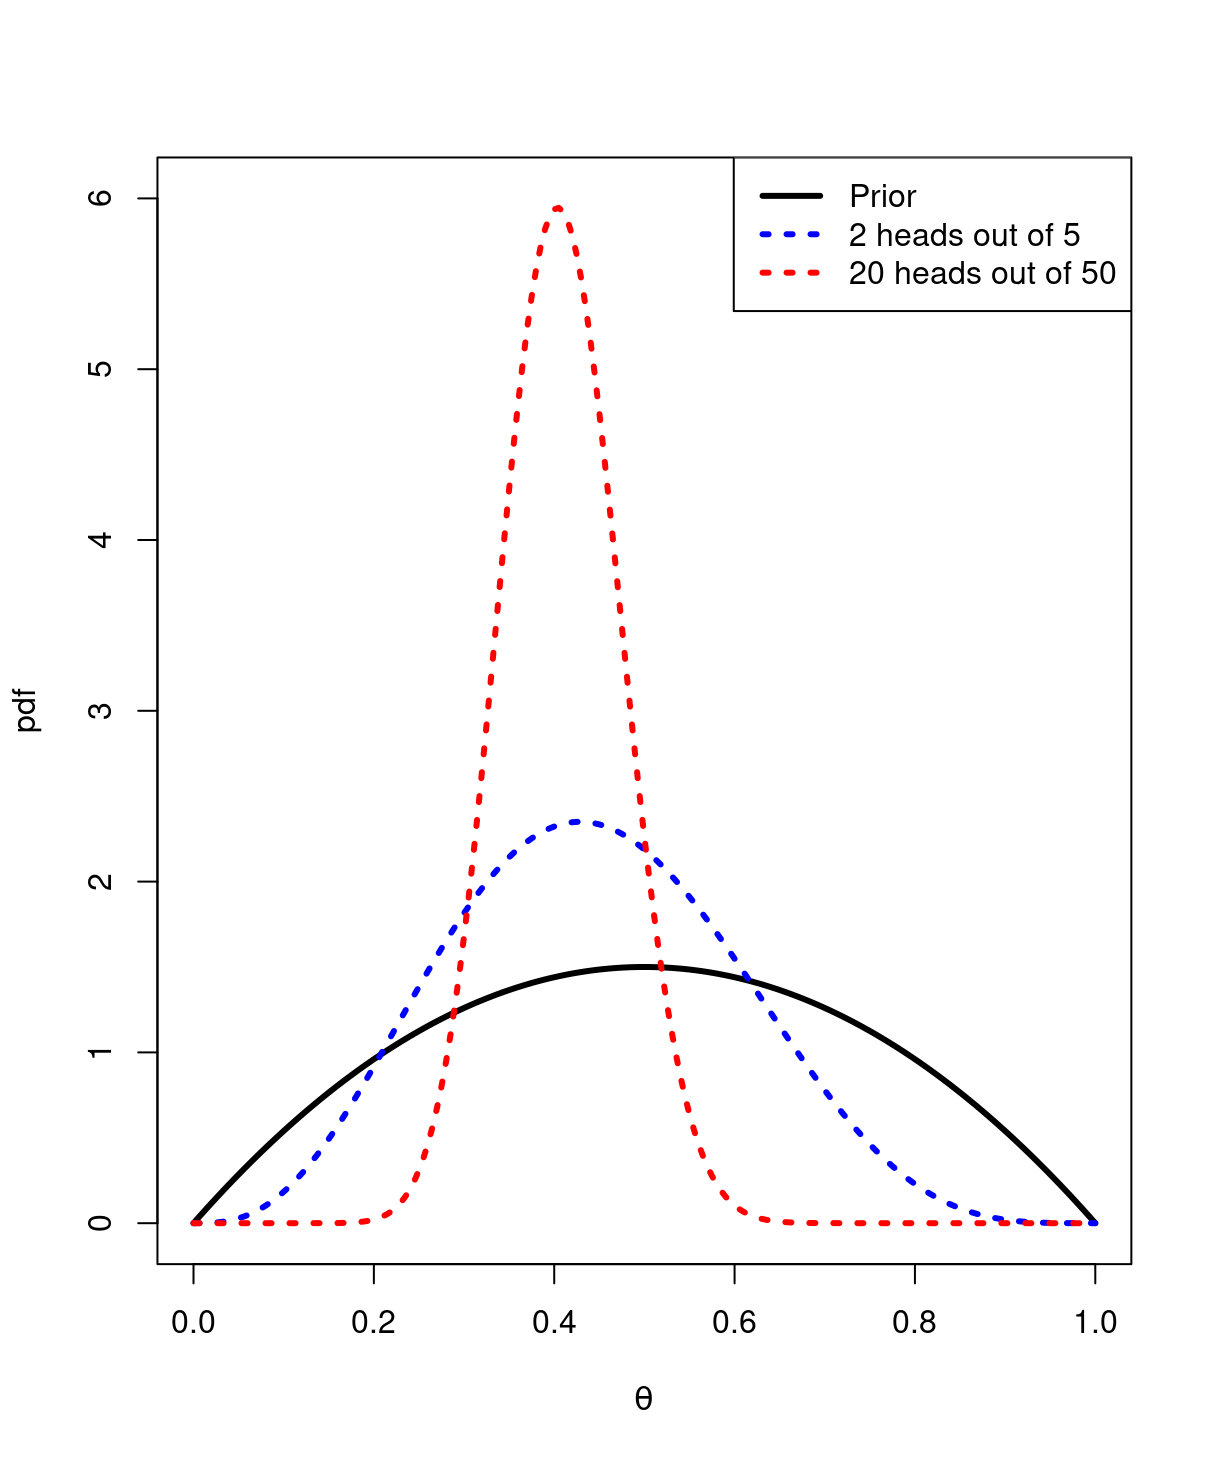
\includegraphics[scale=0.6]{3b.png}
    
    Figure 1: The posterior distributions of $\theta$
\end{center}

The posterior distribution's spread will get smaller and smaller, centered at 
$\theta = 0.4$.

\end{document}
